% Source : http://tex.stackexchange.com/questions/3892/how-do-you-draw-the-snake-arrow-for-the-connecting-homomorphism-in-the-snake-l

\documentclass{article}
\thispagestyle{empty}
\usepackage{amsmath}
\usepackage{tikz}
\usetikzlibrary{%
  matrix,%
  calc,%
  arrows%
}

\DeclareMathOperator{\coker}{coker}

\begin{document}
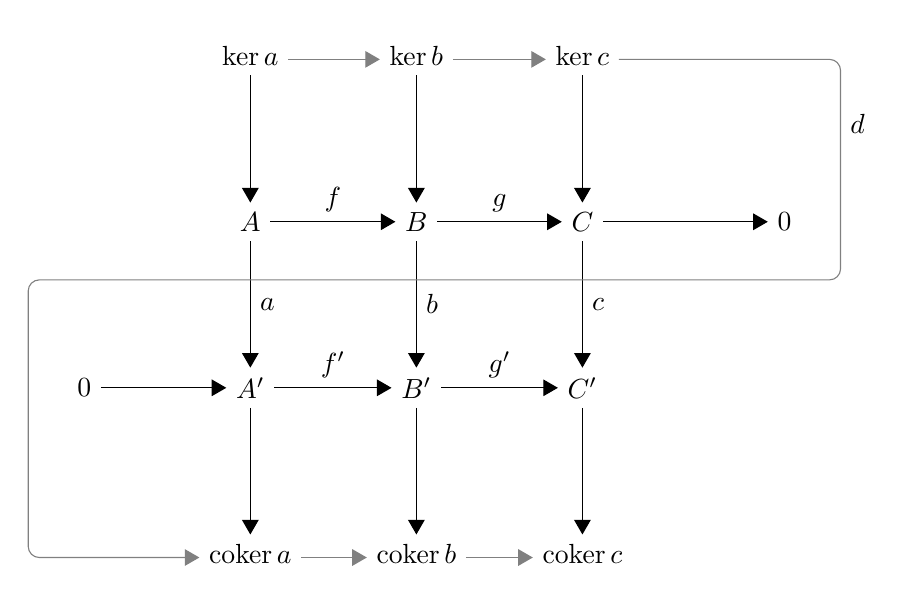
\begin{tikzpicture}[>=triangle 60]
\matrix[matrix of math nodes,column sep={60pt,between origins},row sep={60pt,between origins},nodes={anchor=center}] (s)
{
&|[name=ka]| \ker a &|[name=kb]| \ker b &|[name=kc]| \ker c \\
%
&|[name=A]| A &|[name=B]| B &|[name=C]| C &|[name=01]| 0 \\
%
|[name=02]| 0 &|[name=A']| A' &|[name=B']| B' &|[name=C']| C' \\
%
&|[name=ca]| \coker a &|[name=cb]| \coker b &|[name=cc]| \coker c \\
};
\draw[->] (ka) edge (A)
          (kb) edge (B)
          (kc) edge (C)
          (A) edge node[auto] {\(f\)} (B)
          (B) edge node[auto] {\(g\)} (C)
          (C) edge (01)
          (A) edge node[auto] {\(a\)} (A')
          (B) edge node[auto] {\(b\)} (B')
          (C) edge node[auto] {\(c\)} (C')
          (02) edge (A')
          (A') edge node[auto] {\(f'\)} (B')
          (B') edge node[auto] {\(g'\)} (C')
          (A') edge (ca)
          (B') edge (cb)
          (C') edge (cc)
;
\draw[->,gray] (ka.mid east) -- (kb.mid west);
\draw[->,gray] (kb.mid east) -- (kc.mid west);
\draw[->,gray] (ca.mid east) -- (cb.mid west);
\draw[->,gray] (cb.mid east) -- (cc.mid west);

\draw[->,gray,rounded corners] (kc.mid east) -| 
  node[auto,text=black,pos=.7] {\(d\)} ($(01.east)+(.5,0)$)
 |- ($(B)!.35!(B')$) -| ($(02.west)+(-.5,0)$) |- (ca.mid west);
\end{tikzpicture}
\end{document}
